\chapter{Algorithms}
\label{algos}

This chapter deals with the two locating methods implemented and investigated in the simulation. In order to perform the localization, as seen in \ref{mpls}, the \gls{cir} obtained needs to be treated in order to extract some useful data. The first section shows such methods. Then, using the extracted peaks, two different localization algorithms are shown, a hard based on the trilateration and a soft based on the comparison of theoretical and realistic \gls{cir}.

\section{Peaks extraction}

A \gls{cir} as shown in \ref{fig:cir_ex1} unfortunately does not exist in the real world, at least, not using the material shown in section \ref{loc_syst}. Firstly, extra peaks will appear, because of the double, triple, etc...  reflections on the walls and furniture of the room. Some peaks caused by diffraction may also appear. People walking or standing into the room will also modify the channel and so the \gls{cir}. Secondly, as previously stated in \ref{dwm1000}, the bandwidth of the DWM1000 is not infinite, occasioning a spatial extension of the different peaks. The evolution from a theoretical "perfect" case to a "real" can be observed in Fig. \ref{fig:peaks_real}.

\begin{figure}[H]
\centering
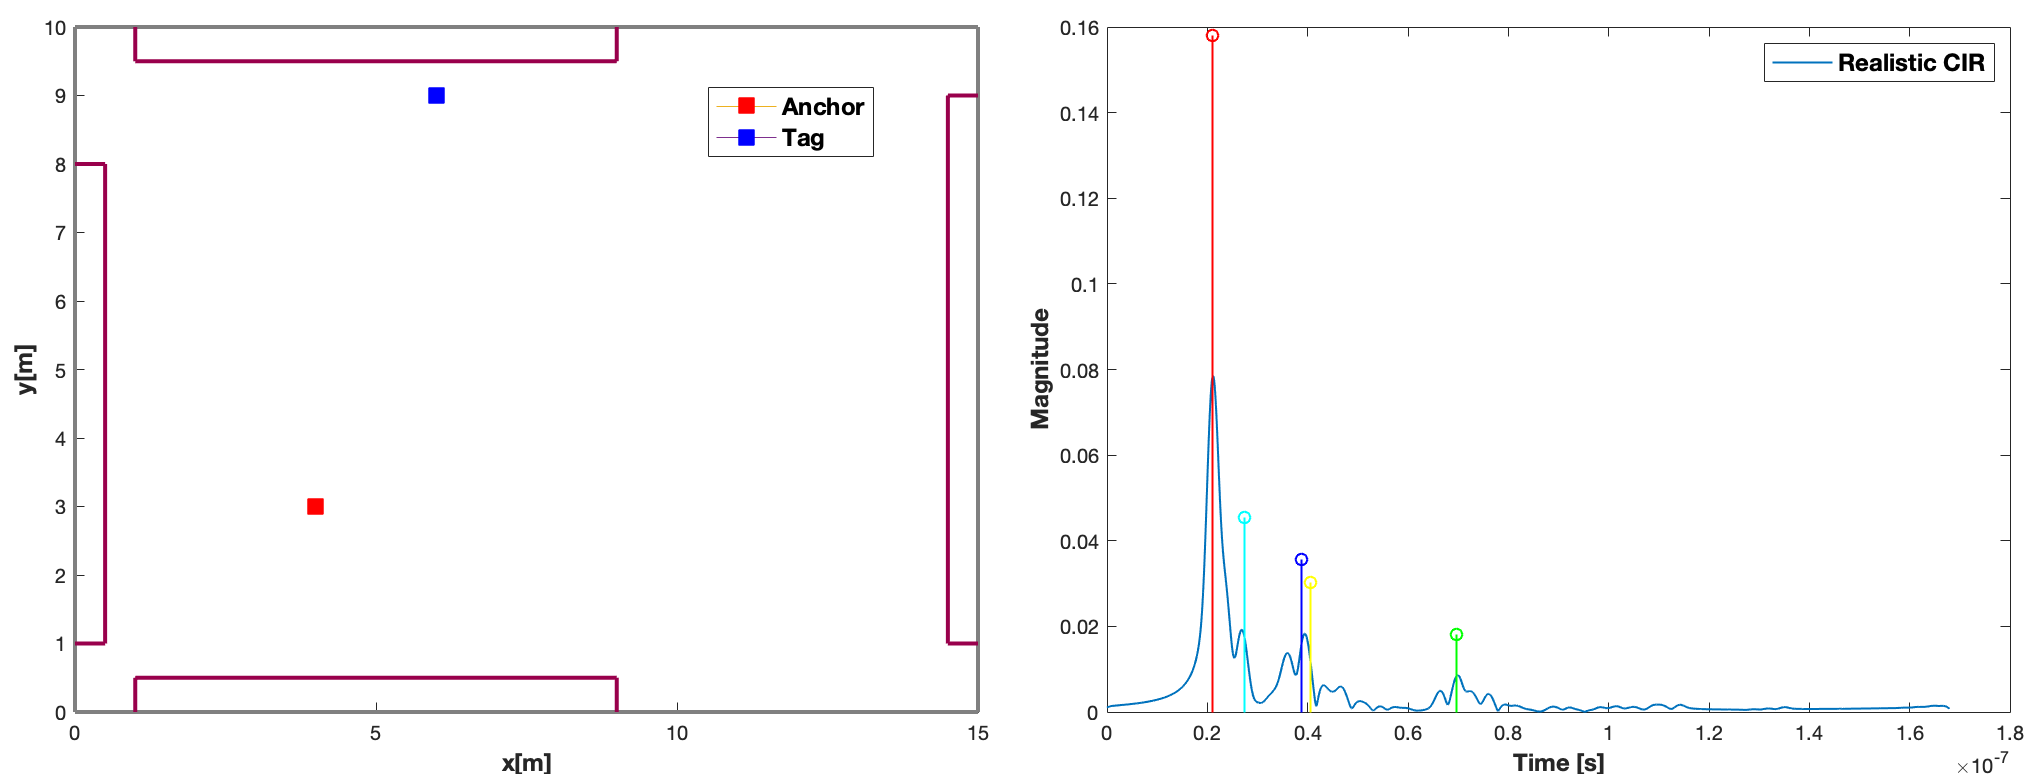
\includegraphics[width=\linewidth]{Images/cir_theo_real.png}
\caption{(Left) Room used to generate the realistic CIR using up to three reflected rays. (Right) Superposition of the CIR in Fig. \ref{fig:UWB_MPC_Theo} and the realistic CIR. \label{fig:peaks_real}}
\end{figure}

The simulation used to generate the realistic \gls{cir} is described in chapter \ref{simulations}. As we can observe, the peaks that originates from the theoretical case matches peaks in the realistic. But can also observe that some new peaks arise in the realistic case, such as those around $0.4*10^{-7}s$. 
\vspace{2mm}

The goal of the peak extraction function is, as the name states, to extract the peaks matching the needs of the locating algorithm. As it will be seen in section \ref{hard_loc}, \ref{soft_loc}, the two methods do not reach their purpose in the same way, the optimal peaks will be slightly different. Hence the two different peaks extraction methods presented below, a soft and a hard case.

\subsection{Soft case}

For the soft locating system, the algorithm of the peak extraction is detailed in algo. \ref{algo:soft}. The algorithm takes as input a vector made of tuples, respectively the time and the amplitude of each point of the \gls{cir}. The $\texttt{n}$ parameter states the number of peaks that the algorithm needs to extract.
\vspace{2mm}

\SetKwInput{KwInput}{Inputs}
\SetKwInput{KwInit}{Initialize}
\SetKwInput{KwOutput}{Output}

\begin{algorithm}[H]
 \KwInput{}\
 \hspace*{\algorithmicindent} $\mathtt{CIR} = \{\mathtt{cir}\} = \{ (\mathtt{t_i}, \mathtt{A_i}) ~\text{s.t.} ~\mathtt{i} \in \mathbb{N}_0\} \in \mathbb{R} \times \mathbb{R}, ~\mathtt{n} \in \mathbb{N}_0$ \;
\KwInit{}
\hspace*{\algorithmicindent} $\texttt{Peaks} \longleftarrow \{ (\mathtt{t_i}, \mathtt{A_i}) ~\text{s.t.} ~\mathtt{i} \in \{ 1, ..., n \} \}$\;
\hspace*{\algorithmicindent} $\texttt{ratio} \longleftarrow \texttt{100}$\;
\hspace*{\algorithmicindent} $\texttt{i} \longleftarrow 1$\;
\hspace*{\algorithmicindent} $\texttt{CIR}_\texttt{max} \longleftarrow \texttt{local\_max}(\texttt{CIR})$\;
\hspace*{\algorithmicindent} $\texttt{CIR}_\texttt{max} \longleftarrow \texttt{Order(CIR}_\texttt{max}\texttt{, 'Descend', 'Prominence based')}$\;


\For{$\texttt{\{cir\}}$ in $\texttt{CIR}_\texttt{max}$}{
	\If{$\texttt{prom(}\texttt{\{cir\})}$ > $\texttt{max(CIR)}/\texttt{ratio}$}{
	$\texttt{Peaks[i]} \longleftarrow \texttt{\{cir\}}$\;
    $\texttt{i} \longleftarrow \texttt{i} + 1$\;
    		\If{$\texttt{i}$ > $\texttt{n}$}{
    		\texttt{break}\;
    		}
	}
 }
 \KwOutput{}\
 \hspace*{\algorithmicindent} $\texttt{Peaks}$\;
 \caption{Peaks Extraction - Soft case \label{algo:soft}}
\end{algorithm}
\vspace{2mm}

During the initialization phase, first, the output \texttt{Peaks} is defined, this variable will be used to store the different extracted peaks. The variable \texttt{i} is the counter of the number of peaks found and stored into the \texttt{Peaks} vector while \texttt{ratio} is used to set a limit to the relative size of the peaks being taken\footnote{This value of 100 is arbitrary, it avoids the program to take really small peaks produced by the noise.}. The local maximum of the \texttt{CIR} is then saved in $\texttt{CIR}_\texttt{max}$ and ordered in the decreasing order based on the prominence of each peak. The definition of the prominence is reminded in Fig. \ref{fig:prominence}. Since the prominence depends on the local minima between two peaks, a higher amplitude does not always imply a higher prominence.

\begin{figure}[H]
\centering
\includegraphics[width=.35\linewidth]{Images/prominence.png}
\caption{Difference between the prominence of a peak and its amplitude \label{fig:prominence}}
\end{figure}

The main loop then gets the $\texttt{n}$ first values of $\texttt{CIR}_\texttt{max}$ and store it into $\texttt{Peaks}$. The $\texttt{If}$ condition is, as said before, used to remove the small fluctuation in the \gls{cir} because of the background, only keeping the most important peaks. If there is less than $\texttt{n}$ peaks that fulfil the conditions, the algorithm returns as many peaks as possible while still respecting the pre-established conditions.

\subsection{Hard case}

For the hard locating system, the same methodology is used. Algorithm \ref{algo:hard} slightly changes at several places. Firstly, the input is only $\texttt{CIR}$, the algorithm always gives back three peaks in $\texttt{Peaks}$. Secondly, the ordering of $\texttt{CIR}_\texttt{max}$ is made based on the amplitude of the peaks. Finally, the amplitude, not the prominence, of the $\{\texttt{cir}\}$  is compared with $\texttt{max(CIR)}/\texttt{ratio}$.
\vspace{2mm}

\begin{algorithm}[H]
 \KwInput{}\
 \hspace*{\algorithmicindent} $\mathtt{CIR} = \{\mathtt{cir}\} = \{ (\mathtt{t_i}, \mathtt{A_i}) ~\text{s.t.} ~\mathtt{i} \in \mathbb{N}_0\} \in \mathbb{R} \times \mathbb{R}$ \;
\KwInit{}
\hspace*{\algorithmicindent} $\texttt{Peaks} \longleftarrow \{ (\mathtt{t_i}, \mathtt{A_i}) ~\text{s.t.} ~\mathtt{i} \in \{ 1, 2, 3 \} \}$\;
\hspace*{\algorithmicindent} $\texttt{ratio} \longleftarrow \texttt{100}$\;
\hspace*{\algorithmicindent} $\texttt{i} \longleftarrow 1$\;
\hspace*{\algorithmicindent} $\texttt{CIR}_\texttt{max} \longleftarrow \texttt{local\_max}(\texttt{CIR})$\;
\hspace*{\algorithmicindent} $\texttt{CIR}_\texttt{max} \longleftarrow \texttt{Order(CIR}_\texttt{max}\texttt{, 'Descend', 'Amplitude based')}$\;


\For{$\texttt{\{cir\}}$ in $\texttt{CIR}_\texttt{max}$}{
	\If{$\texttt{amp(}\texttt{\{cir\})}$ > $\texttt{max(CIR)}/\texttt{ratio}$}{
	$\texttt{Peaks[i]} \longleftarrow \texttt{\{cir\}}$\;
    $\texttt{i} \longleftarrow \texttt{i} + 1$\;
    		\If{$\texttt{i}$ > $\texttt{3}$}{
    		\texttt{break}\;
    		}
	}
 }
 \KwOutput{}\
 \hspace*{\algorithmicindent} $\texttt{Peaks}$\;
 \caption{Peaks Extraction - Hard case \label{algo:hard}}
\end{algorithm}
\vspace{2mm}


\section{Hard localization algorithm}
\label{hard_loc}
This locating system is based on the idea of trilateration and tries to imitate it. Using three peaks, it tries to match those with the anchor and two \glspl{va} to find an intersection point as in the Fig. \ref{fig:trilateration}. Those three peaks are extracted with the algorithm \ref{algo:hard} from the received \gls{cir} at the tag. First, the number of systems that need to be solved is shown, then a systematic method to solve them is suggested.

\subsection{Virtual antennas combination}

The hypothesis that the greatest peak, which is usually the first one, corresponds to that from the \gls{los} ray is made, this implies that there always exists a \gls{los} in those rooms, meaning that this does not suffer from attenuation. About the second and third peak, since each can not be surely associated with a \gls{va}, the only available solution is to try every combination of \glspl{va}. The order being important\footnote{Associating the tuple $(d_1, d_2)$ to $(va_1, va_2)$ is not equivalent to associate it to $(va_2, va_1)$.}, there are $P^2_4 = \frac{4!}{2!} = 12$ different systems to solve. This computation has been made for a room with a simple rectangular geometry. Of course, with a more complex geometry, the number of possible combinations would increase.
\vspace{2mm}

On Fig. \ref{fig:va_sym}, a possible problem is shown. The \gls{cir} shown on the left side is obtained by computing only the \gls{los} and the first reflections onto the different walls. In theory, five different peaks should be seen, but only four appear. In this particular case, the second peak is formed by the peaks from the blue \gls{va} and the green \gls{va}, which will be undistinguishable.

\begin{figure}[H]
\centering
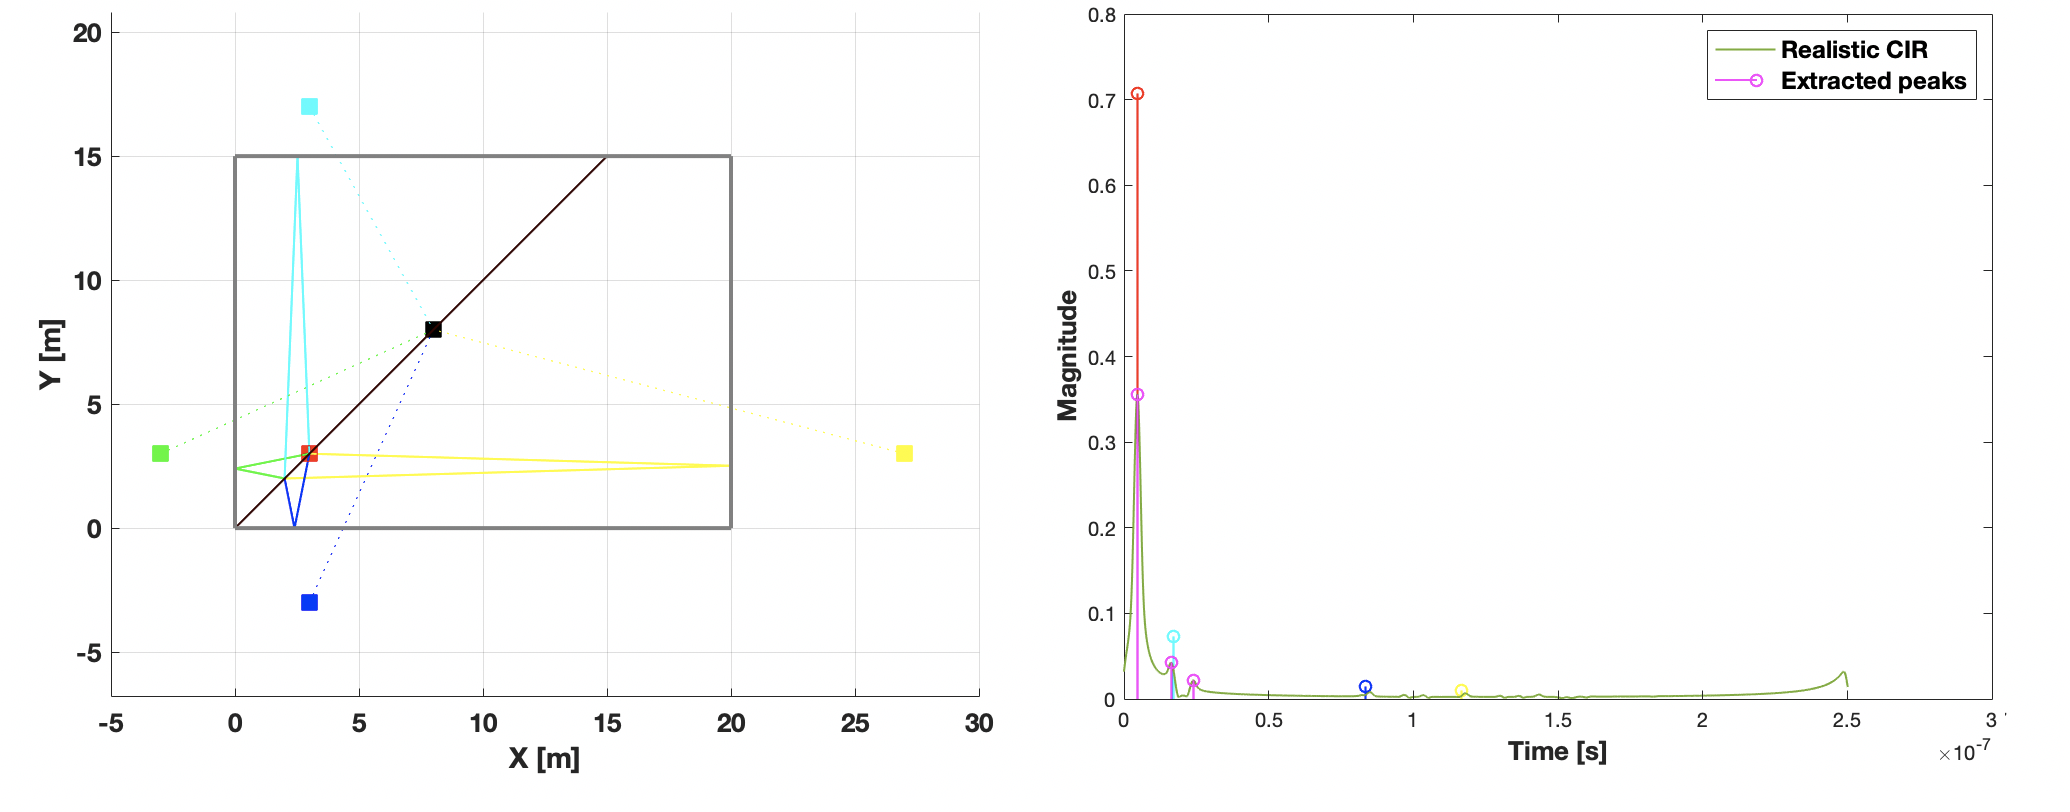
\includegraphics[width=\linewidth]{Images/antenna_combined.png}
\caption{(Left) Room with the anchor in red and the tag in black. (Right) CIR corresponding to the room in the left image, the color of the peaks match the color of the associated VAs. The magenta peaks corresponds to those extracted using the algo. \ref{algo:hard} from the realistic CIR in green. \label{fig:va_sym}}
\end{figure}

A problem that may arise in such situation is that the peaks taken from the \gls{cir} could not correspond to some actual theoretical peaks\footnote{The one that corresponds to one reflection. }. Such an example can be seen on the right image in  Fig. \ref{fig:va_sym} where the third magenta peak does not correspond to any theoretical peak. To overcome this problem, the proposed solution is to consider the peaks as mingled. Hence to the twelve possible combinations discussed , we would have to consider that the second magenta peak originates from two different \glspl{va}, as the cyan peak on the right image of Fig \ref{fig:va_sym}.
\vspace{2mm}

This method has the disadvantage of requiring much computation since twelve more peaks - \glspl{va} need to be checked, but it will solve some symmetry-related problems. This kind of problem can mostly be occurring when the tag is equidistant from two \glspl{va}\footnote{As on the brown line on the map, being the axial symmetry between the two bottoms and left \glspl{va}.}. Since this peak combination due to the tag being equidistant to two \glspl{va} only occurs some specific cases, we should first check the original antenna combination before checking those added.
\vspace{2mm}

Another source of trouble for this algorithm is the finite bandwidth of the antennas. As it can be seen on Fig. \ref{fig:inftofin}, peaks that can be distinguished on the theoretical \gls{cir} are mingled in the realistic. This phenomenon can be observed with the blue and the cyan peaks for example, which are so close that there are considered as one in the finite band \gls{cir}.

\begin{figure}[H]
\centering
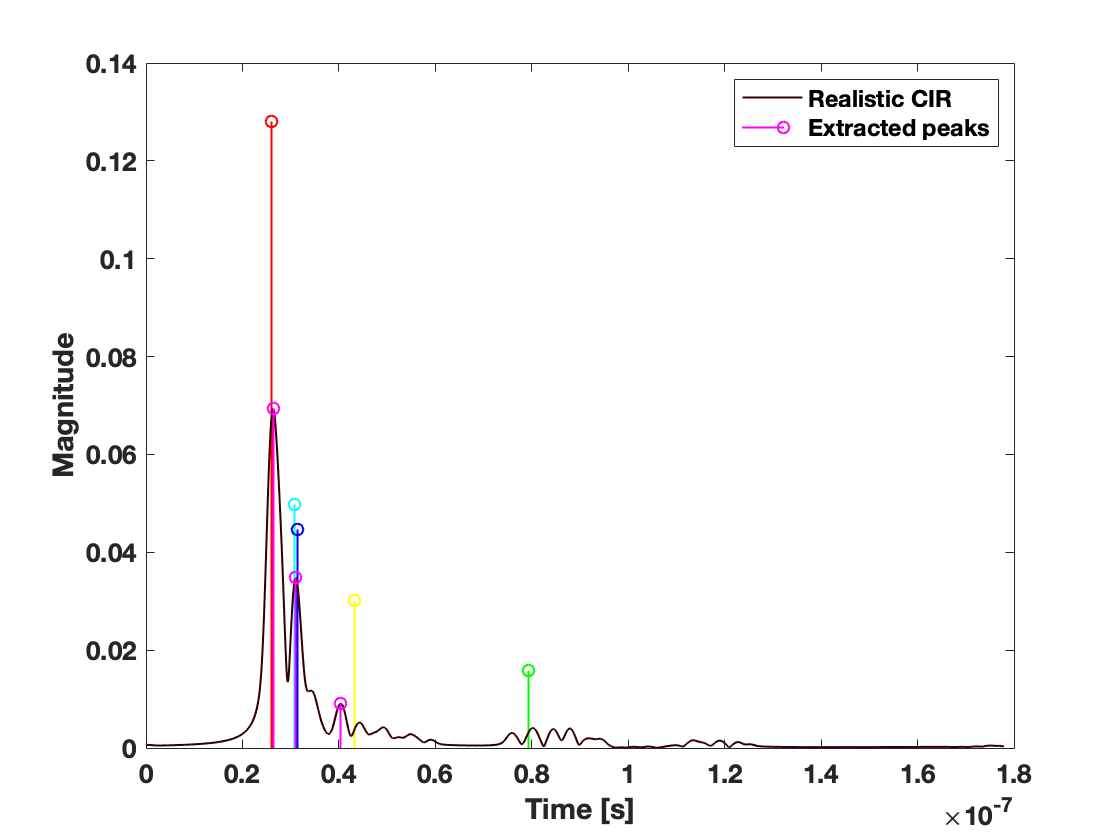
\includegraphics[width=.55\linewidth]{Images/Fig_inf_to_fin.png}
\caption{Infinite bandwidth CIR generated and the finite bandwidth associated in brown. The extracted peaks are shown in magenta. \label{fig:inftofin}}
\end{figure}

To deal with this peak merging issue, the solution proposed is the same that deals with peaks occurring from two \glspl{va} equidistant from the tag. The precision achieved on the localization in such case would be reduced  in those cases. Such examples will be shown in chapter \ref{simulations}. Of course, the third detected peak could also originate from a \gls{va} after a simple reflection, this discussion only make sense when it does not.
\vspace{2mm}

\subsection{System solver}

Those systems are solved one at a time, starting with the twelve 'basic', going on with the particular cases shown above if no suitable solution has been found. Since there is almost no chance that the system leads into a perfect one point solution, the system \ref{eq:syst_exact} can not simply be resolved. The three equations are solved two by two, giving six real or complex solutions. If the six computed intersection belongs to the Real, this would correspond to $U_{12}, U_{13}, U_{23}$ and the Tag\footnote{The position of the tag should appears 3 times, one for each combination of anchors.} in Fig. \ref{fig:trilateration}. From this point, the algorithm first excludes the solutions lying out of the room, the solutions having an imaginary part are also discarded. 
\vspace{2mm}

Using the remaining solutions, the algorithm needs to check if those can be combined to find a suitable solution. A solution is considered as suitable if the algorithm can find three solutions being relatively close to each other. This notion of "relatively close" is subjective and is one of the parameter that we can use to tune the algorithm. If no solution is found using all the combinations, then no location is provided, hence the qualification of "hard".
\vspace{2mm}

\section{Soft localization algorithm}
\label{soft_loc}

The locating system shown in this section reaches localization by comparing some theoretical \gls{cir}, computed by knowing the geometry of the room with the \gls{cir} recovered at the tag. In order to make this comparison, the room is sampled, based on the wished precision we would like to reach. In this thesis, the sample will be made using square of one meter side.
\vspace{2mm}

For each peak extracted from the \gls{cir}, two informations are available, the time of arrival of this peak and its amplitude. We could use the amplitude of the peaks, this would probably work in a lot of cases in the simulation, but this approach has a major drawback: while the peaks are more likely arrive a the same time in both cases, their amplitude can not be guaranteed.
\vspace{2mm}

For example, if a peak suffers from too much attenuation in the real case compared with the simulation, because of losses coming from the transmission, due to reflections on the different materials which are not perfectly simulated, due to a not perfectly isotropic emission of the antenna in the room plane, etc. All those reasons may vary the amplitude of each peak of the \gls{cir}, meaning that nothing can ensure that the proportionality between the \gls{los} peak and the other peaks would be conserved as in the simulation.
\vspace{2mm}

For those reasons, the comparison will be based on the time-of-arrival of each peak. This method also has some drawbacks, the transition to the finite band does not ensure that the peaks will remain at their exact locations. When two peaks mingle, the new peak remaining in finite band iare more likely to have an arrival in the middle of those two peaks. Some precautions have been taken to minimize the errors induced by this phenomenon.
\vspace{2mm}

\subsection{Space solution reduction}

Since the algorithm needs to compare the theoretical \gls{cir} with every possible position of the tag, in order to speed-up the program, we could actually reduce the number of locations to test.
\vspace{2mm}

Using the \gls{sdstwr}, the \gls{tof} of the signal between the tag and the anchor can be computed\footnote{In the simulation, it will be assumed to be extracted from the \gls{cir}}. Based on this \gls{tof}, a circle drown be traced with the center on this anchor and the radius being the estimated distance deduced from the \gls{tof}. In theory, the tag is supposed to be located on this circle, but because of the discretization and errors on the \gls{tof}, a margin is taken to get the set of possible locations. This margin lies in the between of the two orange circles, that can be observed on Fig. \ref{fig:speedup_1}.
\vspace{2mm}

\begin{figure}[H]
\centering
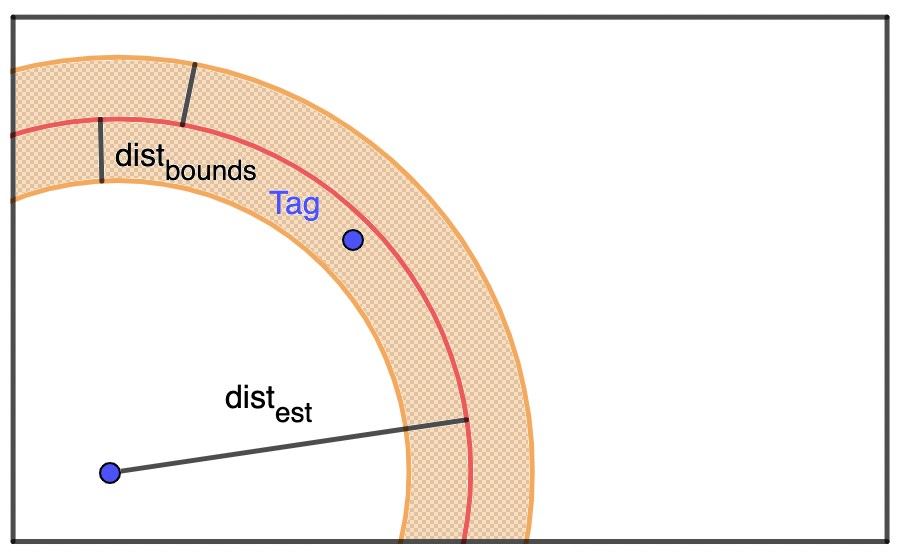
\includegraphics[width=.65\linewidth]{Images/algo_1.png}
\caption{Example of the application of the space solution reduction. The remaining space solution is shown in orange.}
\label{fig:speedup_1}
\end{figure}

From the position inside those boundaries, a mask matrix representing all the positions of the room is filled with ones for the position inside of the orange zone. The other positions are left to zero. Later, this mask is used to reduce the computations since only the values associated with a one will be tested.
\vspace{2mm}

This will lead to a matrix, of witch the size depends on the chosen discretization of the room, filled with one and zero. The meaning of a one in this matrix means that the location associated to this entry of the matrix has been judged as a probable location for the tag. Therefore, the next step of this algorithm is performed only at those locations. This results are in a map as displayed in Fig. \ref{fig:mse_example} where only an arc has been evaluated, not the wall map.

\subsection{Time MSE}

For each remaining possible location, a finite band \gls{cir} is simulated using only the direct and the single reflected rays. Such example can be found in Fig. \ref{fig:soft_simu}. In order to obtain something similar to the realistic case, the \gls{cir} has been passed in the finite band. The peaks are then extracted using algo. \ref{algo:soft} from this finite band \gls{cir}.

\begin{figure}[H]
\centering
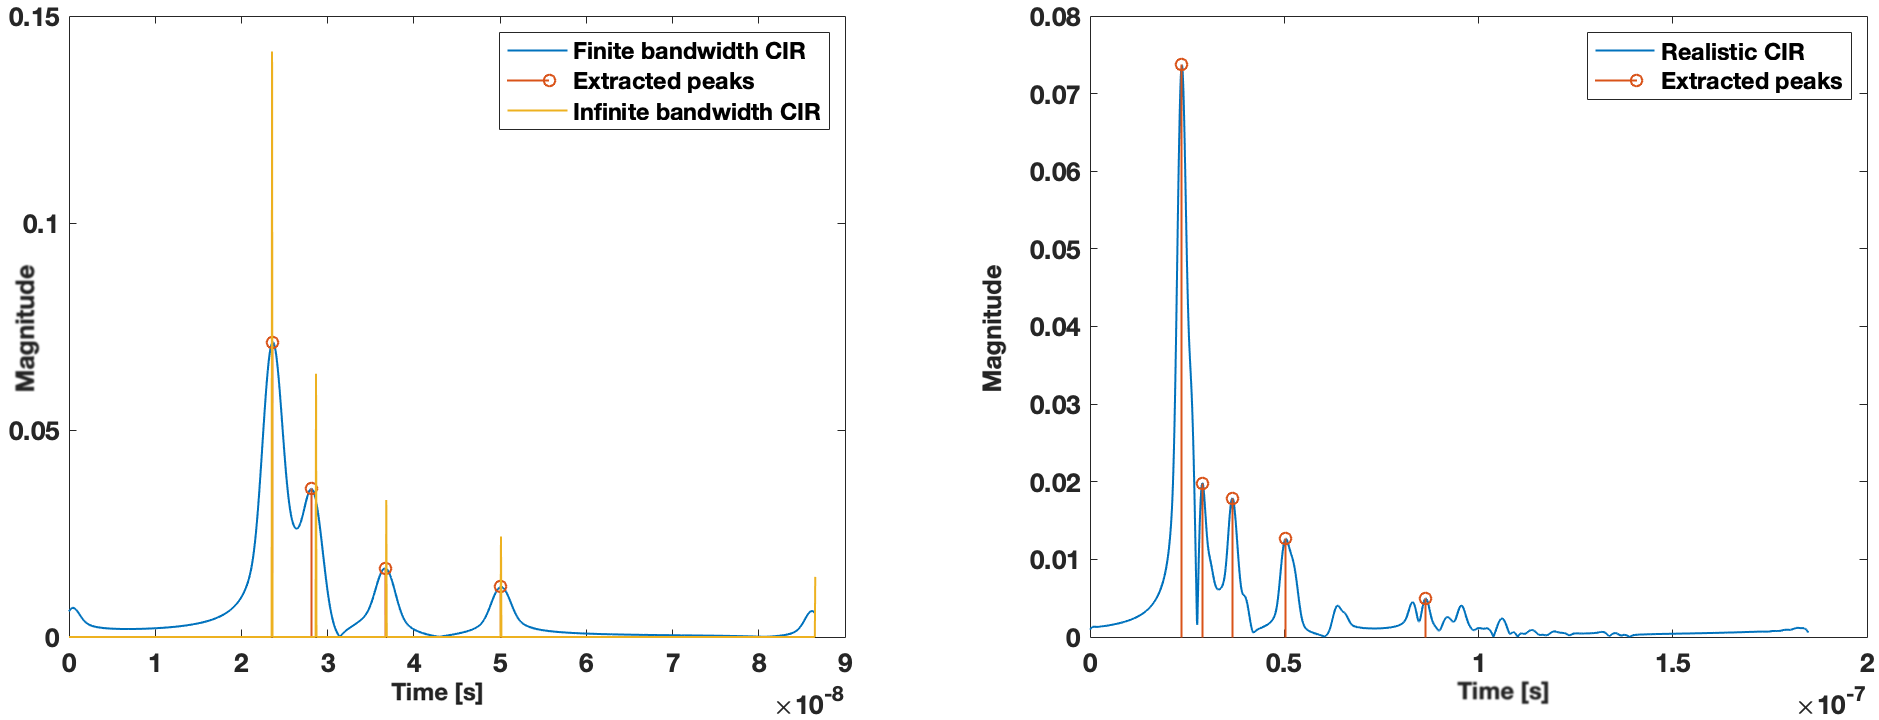
\includegraphics[width=\linewidth]{Images/inf_vs_fin.png}
\caption{(Left) Theoretical CIR obtained using the simulation. The same room has been used as for the right image, without furniture and using only the direct ray and single reflected rays.  (Right) Realistic CIR obtained in a room full of furniture using the simulation.\label{fig:soft_simu}}
\end{figure}

The extraction is also done once on the \gls{cir}. By use of the different peaks extracted, the following problem is solved. 

\begin{equation}
\label{eq:mse_time}
\begin{aligned}
S(\vec{p_0}) &= \sum_i^N (\|\text{Peaks}(\vec{p_{r}})_i - \text{Peaks}(\vec{p_{0}})_i\| ^2 ) \\
\vec{p_0} &= \underset{\vec{p}}{\text{argmin}}~ S(\vec{p})
\end{aligned}
\end{equation}

The peaks extracted are sorted in the chronological order in the peak extraction. Therefore, the sum goes through the peaks of both \gls{cir}. The argument $\text{N}$ is limited by the smallest list of peaks given by the algo. \ref{algo:soft}. While the $\vec{p_0}$ represents all the possible positions tested, $\vec{p_r}$ represents the real cases. $\text{Peaks}(\vec{p_0})_i$ represents the $i^{th}$ peak extracted from the theoretical \gls{cir} computed by placing the tag at the position $\vec{p_0}$.
\vspace{2mm}

This algorithm will have as output a map of the room with the \gls{mse} of the time arrival of the peaks computed at each possible location. An example of such output can be seen in Fig. \ref{fig:mse_example}, this heat-map has been generated using the \gls{mse} computed at each location evaluated. The estimator from eq. \ref{eq:mse_time} will provide only one output, being the one with the lowest \gls{mse}. A solution will always be provided by this locating system. 
\vspace{2mm}

\begin{figure}[H]
\centering
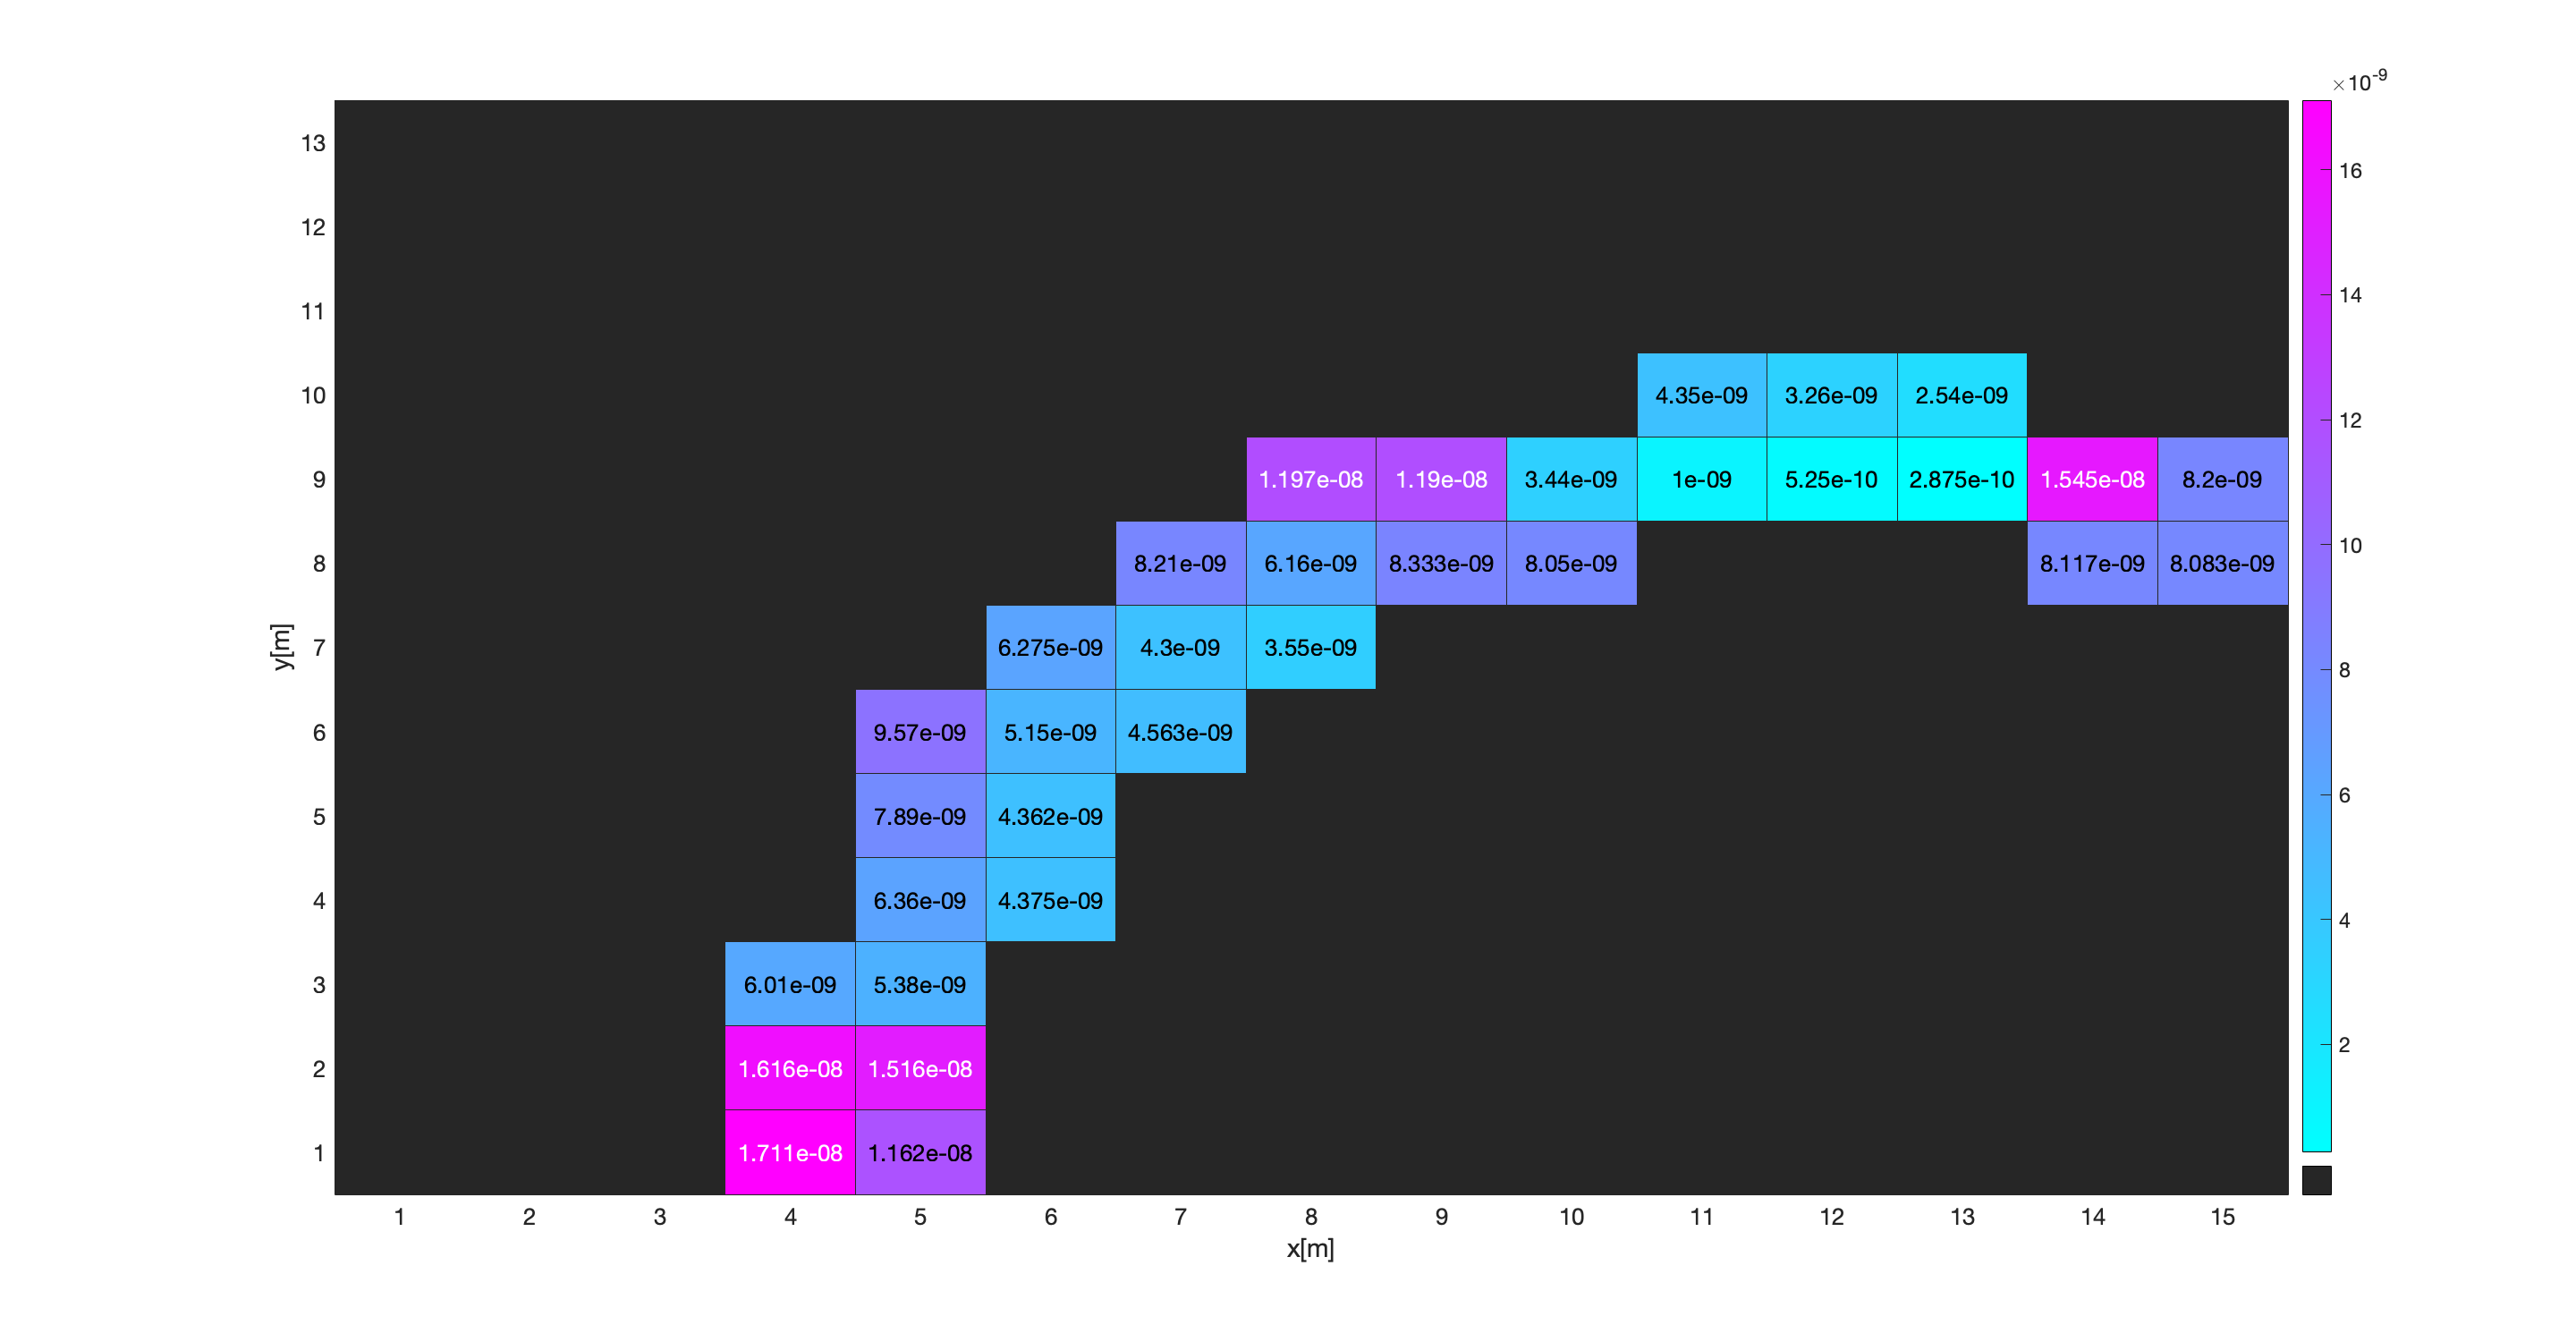
\includegraphics[width=\linewidth]{Images/mse_map_algo.png}
\caption{Example of an execution of the soft localization algorithm. Anchor at (12,2) and Tag at (13,9).\label{fig:mse_example}}
\end{figure}

The locations that were not estimated because of the space solution reduction occurring before the computation of the \gls{mse} are colored in black.